\documentclass[10pt]{beamer}
\usepackage{amsmath,amsfonts,microtype,nicefrac,amssymb, amsthm,centernot}
\usefonttheme{professionalfonts}
\usefonttheme{serif}

\usepackage{palatino}
\usepackage{mathpazo} % or: {newpxtext,newpxmath}
\renewcommand\familydefault{\rmdefault}

\usepackage[utf8]{inputenc}
\usepackage[T1]{fontenc}
\usepackage{textcomp}
\usepackage{bm}

\usepackage{tikz}
\usetikzlibrary{arrows.meta}
\usetikzlibrary{positioning}
\usetikzlibrary{arrows,shapes}
\usepackage{caption, subcaption}

%% BEAMER BUTTON
%\setbeamertemplate{button}{\tikz
%\node[
%	inner xsep = 2pt, 
%	draw = structure!0, 
%	fill = myblue, 
%	rounded corners = 4pt]{\color{white} \tiny\insertbuttontext};
%}


%% ALGORITHM 
\usepackage{algorithm}
\usepackage[noend]{algpseudocode}
\usepackage{multimedia}

%% THEME
\usetheme[frametitleformat=regular,titleformat=regular]{Madrid}
\setbeamerfont{frametitle}{shape=\normalfont}
\setbeamerfont{title}{shape=\normalfont}

%% PATHS
\graphicspath{{./results/}}
\makeatletter
\def\input@path{{../draft/tables/latexData/}}
\makeatother

%% FIGURE ENVIRONMENT 
\usepackage{booktabs,siunitx}

\usepackage{pgfplots} 
%\usepackage[outdir=./figures]{epstopdf}
\usepackage{epstopdf}
\usepackage{float}
\usepackage{graphicx}

\usepackage[absolute,overlay]{textpos}

%% COLORS
%% LINKS
\definecolor{myred}{RGB}{163,32,45}
\definecolor{navyblue}{rgb}{0.05,0.2,0.70}
\definecolor{myblue}{RGB}{0,51,150}
\definecolor{myorange}{RGB}{255,140,0}
\definecolor{myref}{RGB}{160,160,160}
\definecolor{shock}{RGB}{0, 125, 34}%{50, 168, 82}

%% TRANSPARENCY

\usepackage{transparent}

%% BEAMER TEMPLATE
\usetheme{Boadilla}

\makeatother
\setbeamertemplate{itemize items}{\large\raisebox{-0.25ex}{\textbullet}}
\setbeamertemplate{itemize subitem}{\footnotesize\raisebox{0.15ex}{--}}
\setbeamertemplate{itemize subsubitem}{\Tiny\raisebox{0.7ex}{$\blacktriangleright$}}
%\setbeamertemplate{itemize subsubitem}{\color{yellow}$\blacksquare$}

\setbeamertemplate{enumerate item}[default]
\setbeamertemplate{enumerate subitem}{\textbullet}
\setbeamertemplate{footline}{}
\makeatletter
\setbeamertemplate{navigation symbols}{}


%% FORMATTING AUTHORS
%\usepackage{authblk}
\usepackage{url}
\usepackage{multirow}
\usepackage{array}

%% FRAME ITEMIZE SPACING
\usepackage{xpatch}

\xpatchcmd{\itemize}
{\def\makelabel}
{\setlength{\itemsep}{2.5ex}\def\makelabel}
{}
{}

\xpatchcmd{\enumerate}
{\def\makelabel}
{\setlength{\itemsep}{10ex}\def\makelabel}
{}
{}

%% APPENDIX 
\usepackage{appendixnumberbeamer}


%% TITLE AND OPENING
\title{\large Lecture 1}
\subtitle{Dynamics: Discrete Time}
\author{Andreas Schaab}
\date{}


\begin{document}
\tikzstyle{every picture}+=[remember picture]
%\everymath{\displaystyle}
\thispagestyle{empty}
\maketitle 
\newpage

\addtocounter{framenumber}{-1}



%%%%%%%%%%%%%%%%%%%%%%%%%%  SLIDE   %%%%%%%%%%%%%%%%%%%%%%%%%%%%%%%%
\begin{frame}{Introduction}
\begin{itemize}
\item Many (most) economic phenomena are about dynamics

\item Dynamics $\sim$ changes in the behavior of economic agents over time

\item This is a course about \textbf{dynamic optimization}: main approach to study dynamic models in economics 

\item Goal of this course: hard skills + empower you to do research

$\implies$ \textit{focus on tools, but with tons of applications }

\item The more you can ``tool up'' during your first two years, the better

\item Specifically: \textbf{dynamic programming} one of most powerful tools in economic analysis

\end{itemize}
\end{frame}


%%%%%%%%%%%%%%%%%%%%%%%%%%  SLIDE   %%%%%%%%%%%%%%%%%%%%%%%%%%%%%%%%
\begin{frame}{Dynamic programming will empower you}
\begin{itemize}
\item Macro: consumption, investment, portfolio allocation, ... 

\item Labor: search, wage bargaining, ... 

\item IO: competition and games, pricing, ...

\item Finance: asset pricing, dynamic capital structure, portfolio choice, ... 

\item Growth: technology adoption, poverty traps, firm innovation, ... 

\item Urban: migration in spatial models, ... 

\item Inequality: evolution of income-wealth distribution, ... 

\item Game theory: dynamic games, ... 

\item ... much, much more 

\end{itemize}
\end{frame}

%%%%%%%%%%%%%%%%%%%%%%%%%%  SLIDE   %%%%%%%%%%%%%%%%%%%%%%%%%%%%%%%%
\begin{frame}{Outline of today's lecture}
\addtocounter{framenumber}{-1}

\begin{itemize}
\item Administrative course overview

\item Dynamics in discrete time
\begin{enumerate}
	\item Stochastic processes
	\item Markov chains
	\item Difference equations
	\item Prominent examples of difference equations in macro
	\item Solow growth model
	\item Stochastic difference equations
\end{enumerate}
\end{itemize}
\end{frame}


%%%%%%%%%%%%%%%%%%%%%%%%%%  SLIDE   %%%%%%%%%%%%%%%%%%%%%%%%%%%%%%%%
\begin{frame}{Acknowledgements}
\begin{itemize}
\item Course builds on excellent teaching material developed by others

\item Huge thanks to David Laibson for making available his incredible course on dynamic programming 

\url{https://projects.iq.harvard.edu/econ2010c/lecturesDLaibson}

\item Benjamin Moll's teaching material and code tutorials are among the best / most pedagogical I know

\url{https://benjaminmoll.com/}

\item Pablo Kurlat has fantastic teaching material online

\url{https://sites.google.com/view/pkurlat/teaching}

\item Many others ... (this slide will evolve)

\item Closest textbooks: Stokey-Lucas, Ljungqvist-Sargent, Acemoglu, Romer

\end{itemize}
\end{frame}


%%%%%%%%%%%%%%%%%%%%%%%%%%  SLIDE   %%%%%%%%%%%%%%%%%%%%%%%%%%%%%%%%
\begin{frame}{GitHub}
\begin{itemize}
\item One super useful \textit{hard skill} for research / code development: \\
version control

\item You should start using git (via GitHub) in your own work from the start

\item Course material will be available via a GitHub organization at:
\url{https://github.com/schaab-teaching/DynamicProgramming}

\item You should create a GitHub account if you don't already have one

\item If this is new for you, I also recommend GitKraken

\item You can get Pro versions of GitHub and GitKraken for free after verifying your academic affiliation

\item Great resource: \url{https://git-scm.com/book/en/v2} \\
(Especially chapters 2, 3, 5, and 6)

\end{itemize}
\end{frame}


%%%%%%%%%%%%%%%%%%%%%%%%%%  SLIDE   %%%%%%%%%%%%%%%%%%%%%%%%%%%%%%%%
\begin{frame}{Admin}
\begin{itemize}
\item Fall semester macro: Andreas + Gerard, then Fabrice + Oscar

\item PSETs every week, solutions will be provided

$\implies$ \textit{You are responsible from now on}

\item Final exam will be close to the PSETs

\item Recommended books:
\begin{itemize}
	\item Ljungqvist and Sargent
	\vspace{-3mm}
	\item Stokey and Lucas
	\vspace{-3mm}
	\item Romer
	\vspace{-3mm}
	\item Acemoglu
	\vspace{-3mm}
	\item Oksendal
	\vspace{-3mm}
	\item LeVeque
	\vspace{-3mm}
	\item Kamien and Schwartz
	\vspace{-3mm}
	\item Stachurski / Miao / ...
\end{itemize}
\end{itemize}
\end{frame}



%%%%%%%%%%%%%%%%%%%%%%%%%%  SLIDE   %%%%%%%%%%%%%%%%%%%%%%%%%%%%%%%%
\begin{frame}{1. Stochastic processes}
\begin{itemize}
\item Let $X_t$ be a random variable that is time $t$ adapted

\item Discrete time: We index time discretely $t = 0, 1, 2, \ldots, T \leq \infty$

\item Stochastic process in discrete time: a sequence of random variables indexed by $t$, $\{X_t\}_{t=0}^T$

\item Continuous time: We index time continuously $t \in [0, T]$ with $T \leq \infty$

\item Stochastic process in continuous time: a sequence of random variables indexed by $t$, $\{X_t\}_{t \geq 0}$

\end{itemize}
\end{frame}



%%%%%%%%%%%%%%%%%%%%%%%%%%  SLIDE   %%%%%%%%%%%%%%%%%%%%%%%%%%%%%%%%
\begin{frame}{2. Markov chains}
\begin{itemize}
\item A stochastic process $\{X_t\}$ has the \textit{Markov property} if for all $k \geq 1$ and all $t$:
\begin{equation*}
	\mathbb P(X_{t+1} = x \mid X_t, X_{t-1}, \ldots, X_{t-k}) = \mathbb P(X_{t+1} = x \mid X_t)
\end{equation*}

\item \textit{State space} of the Markov process = set of events or states that it visits 

\item A Markov chain is a Markov process (stochastic process with Markov property) that visits a finite number of states (\textit{discrete state space})

\item Simplest example: Individual $i$ is randomly hit by earnings (employment) shocks and switches between $X_t \in \{X^L, X^H\}$
\end{itemize}
\end{frame}


%%%%%%%%%%%%%%%%%%%%%%%%%%  SLIDE   %%%%%%%%%%%%%%%%%%%%%%%%%%%%%%%%
\begin{frame}{}
\begin{itemize}
\item Markov chains have a \textit{transition matrix} $P$ that describes the probability of transitioning from state $i$ to state $j$

\item Simplest example with state space $\{X^L, X^H\}$
\begin{equation*}
	P = \begin{pmatrix} 0.8 & 0.2 \\ 0.2 & 0.8 \end{pmatrix}
\end{equation*}

\item This says: P of staying in employment state = $0.8$, P of switching = $0.2$

\item $P_{ij}$ is the probability of switching from state $i$ to state $j$ (one period)

\item $P^2$ characterizes transitions over two periods: $(P^2)_{ij}$ is prob of going from $i$ to $j$ in two periods

\item The rows of the transition matrix have to sum to $1$ (definition of probability measure)
\end{itemize}
\end{frame}



%%%%%%%%%%%%%%%%%%%%%%%%%%  SLIDE   %%%%%%%%%%%%%%%%%%%%%%%%%%%%%%%%
\begin{frame}{3. Difference Equations}
\begin{itemize}
\item We start with deterministic (non-random) dynamics and then conclude with stochastic (random) dynamics

\item The \textit{first-order linear difference equation} is defined by
\begin{equation}\label{eq:linear_difference}
	x_{t+1} = b x_t + c z_t 
\end{equation}
where $\{z_t\}$ is an exogenously given, bounded sequence

\item For now, all objects are (real) scalars (easy to extend to vectors and matrices)

\item Suppose we have an \textit{initial condition} (i.e., given initial value) $x_0$

\item When $c = 0$, \eqref{eq:linear_difference} is a \textit{time-homogeneous} difference equation

\item When $cz_t$ is constant for all $t$, \eqref{eq:linear_difference} is an \textit{autonomous} difference equation

\end{itemize}
\end{frame}


%%%%%%%%%%%%%%%%%%%%%%%%%%  SLIDE   %%%%%%%%%%%%%%%%%%%%%%%%%%%%%%%%
\begin{frame}{Autonomous equations}
\begin{itemize}
\item Consider the autonomous equation with $z_t = 1$ 

\item A particular solution is the constant solution with $x_t = \frac{c}{1-b}$ when $b \neq 1$

\item Such a point is called a \textit{stationary point} or \textit{steady state}

\item General solution of the autonomous equation (for some constant $x$):
\begin{equation}\label{eq:linear_difference_solution}
	x_t = (x_0 - x) b^t + x
\end{equation}

\item Important question is long-run behavior (stability / convergence)

\item When $| b | < 1$, \eqref{eq:linear_difference_solution} converges asymptotically to steady state $x$ for any initial value $x_0$ (steady state $x$ is globally stable) 

\item If $| b | > 1$, \eqref{eq:linear_difference_solution} explodes and is not stable (except when $x_0 = x$)
\end{itemize}
\end{frame}



%%%%%%%%%%%%%%%%%%%%%%%%%%  SLIDE   %%%%%%%%%%%%%%%%%%%%%%%%%%%%%%%%
\begin{frame}{4. Difference Equations: Examples in Macro}

\textbf{Capital accumulation}:
\begin{equation*}
	K_{t+1} = (1 - \delta) K_t + I_t
\end{equation*}
\begin{itemize}
\item $\delta$ is depreciation and $I_t$ is investment

\item This is a \textit{forward equation} and requires an initial condition $K_0$

\item If $I_t = 0$ and $0 < \delta < 1$, $K_t \to 0$

\item If $I_t = c$ constant, then $K_t$ converges to $\frac{c}{\delta}$: $K_{t+1} = (1-\delta) \frac{c}{\delta} + c = \frac{c}{\delta}$
\end{itemize}
\end{frame}


%%%%%%%%%%%%%%%%%%%%%%%%%%  SLIDE   %%%%%%%%%%%%%%%%%%%%%%%%%%%%%%%%
\begin{frame}{}
\textbf{Wealth dynamics}:
\begin{equation*}
	a_{t+1} = R_t a_t + y_t - c_t
\end{equation*}
\begin{itemize}
	\item $R_t$ is the gross real interest rate, $y_t$ is income, $c_t$ is consumption
	
	\item This is a \textit{forward equation} and requires an initial condition $a_0$
	
	\item We will study this as a \textit{controlled} process because $c_t$ will be chosen optimally
	
	\item Work out the following: $R_t = R$ and $y_t = y$ constant, and  
	\begin{equation*}
		c_t = \bigg( 1 - \frac{1}{R} \bigg) \bigg(a_t + \sum_{s=t}^\infty R^{-(t-s)} y \bigg)
	\end{equation*}
	What are the dynamics of $a_t$?
\end{itemize}
\end{frame}


%%%%%%%%%%%%%%%%%%%%%%%%%%  SLIDE   %%%%%%%%%%%%%%%%%%%%%%%%%%%%%%%%
\begin{frame}{}
\textbf{Consumption Euler equation}:
\begin{equation*}
	\frac{1}{C_t} = \beta R_t\frac{1}{C_{t+1}}
\end{equation*}
\begin{itemize}
	\item $\frac{1}{C_t} = u'(C_t)$ is marginal utility with log preferences
	
	\item This is a \textit{backward equation} and requires a terminal condition or transversality condition, i.e., $c_T$ must converge to something
	
	\item Suppose there exists time $T$ s.t. for all $t \geq T$, $C_t = C$
	
	\item Then solve \textit{backwards} from: $\frac{1}{C_{T-1}} = \beta R_{T-1} \frac{1}{C_T}$ or expressed as \textit{time-homogeneous first-order linear difference equation}
	\begin{equation*}
		C_{T-1} = \frac{1}{\beta R_{T-1}} C_T
	\end{equation*}

	\item Difference between \textit{forward} and \textit{backward} equations is critical! This is closely related to the idea of \textit{boundary conditions} (much more to come)
\end{itemize}
\end{frame}



%%%%%%%%%%%%%%%%%%%%%%%%%%  SLIDE   %%%%%%%%%%%%%%%%%%%%%%%%%%%%%%%%
\begin{frame}{}
\textbf{New Keynesian Phillips curve}:
\begin{equation*}
	\pi_t = \beta \pi_{t+1} + \kappa x_t
\end{equation*}
\begin{itemize}
	\item $\pi_t$ is inflation, $\kappa$ is the slope of the PC, $x_t$ is output gap
	
	\item This is a \textit{backward equation} and requires a terminal condition
	
	\item NK analysis often studies the case $\lim_{T \to \infty} \pi_T = 0$ ($0$ inflation steady state)
	
	\item Suppose output gap $\{ x_t \}$ exogenously given and there exists $T$ s.t. for $t \geq T$, $\pi_t = 0$ and $x_t = 0$
	
	\item Then we solve backwards: $\pi_{T-1} = \beta \pi_T + \kappa x_{T-1}$
	
	\item The \textit{initial value} $\pi_0$ is \textit{endogenous}: backward equations solve for initial value $\pi_0$, forward equations solve for long run (e.g., $K_T$)
\end{itemize}
\end{frame}



%%%%%%%%%%%%%%%%%%%%%%%%%%  SLIDE   %%%%%%%%%%%%%%%%%%%%%%%%%%%%%%%%
\begin{frame}{5. Solow Growth Model}
\begin{itemize}
\item Time is discrete and the horizon infinite, $t = 0, 1, 2, \ldots$

\item There is a \textit{representative household}: large number of small but identical households

\item Assume households have a constant savings rate $s \in (0, 1)$ (out of disposable income)

\item A representative firm operates the technology / production function
\begin{equation*}
	Y_t = F(K_t, L_t, A_t)
\end{equation*}
where $K_t$ is capital, $L_t$ is labor, $A_t$ is total factor productivity (TFP)

\item Capital accumulation: $K_{t+1} = (1-\delta) K_t + I_t$

\item Goods market clearing (\textit{national income accounting identity}): $Y_t = C_t + I_t$
\end{itemize}
\end{frame}


%%%%%%%%%%%%%%%%%%%%%%%%%%  SLIDE   %%%%%%%%%%%%%%%%%%%%%%%%%%%%%%%%
\begin{frame}{}
\begin{itemize}
\item Feasible allocations in this economy are characterized by
\begin{equation*}
	K_{t+1} \leq F(K_t, L_t, A_t) + (1-\delta)K_t - C_t 
\end{equation*}

\item How do we determine the equilibrium allocation among all those allocations that are feasible? $\implies$ assume constant savings rate
\begin{align*}
	s Y_t &= S_t \\
	&= I_t = Y_t - C_t
\end{align*}
or $C_t = (1-s) Y_t$

\item Equilibrium characterized by (non-linear) first-order difference equation:
\begin{equation}\label{eq:solow}
	K_{t+1} = s F(K_t, L_t, A_t) + (1-\delta) K_t
\end{equation}
\end{itemize}

\textbf{Definition.} (Equilibrium) Given sequences $\{L_t, A_t\}_{t=0}^\infty$ and an initial condition for capital $K_0$, the equilibrium path of the Solow growth model comprises paths for capital, output, consumption and investment $\{K_t, Y_t, C_t, I_t\}_{t=0}^\infty$ that satisfy \eqref{eq:solow}, goods market clearing, firm production, and $C_t = sY_t$.
\end{frame}


%%%%%%%%%%%%%%%%%%%%%%%%%%  SLIDE   %%%%%%%%%%%%%%%%%%%%%%%%%%%%%%%%
\begin{frame}{Steady state}
\begin{itemize}
\item Suppose Cobb-Douglas technology:
\begin{equation*}
	Y_t = A K_t^\alpha L_t^{1-\alpha}
\end{equation*}
and no productivity or population growth; also normalize $L_t = 1$

\item A steady state is a level of capital $K$ such that 
\begin{equation*}
	K = s A K^\alpha + (1-\delta) K
\end{equation*}

\item Solving this, we find:
\begin{equation*}
	K = \bigg(\frac{sA}{\delta}\bigg)^\frac{1}{1-\alpha}
\end{equation*}
\end{itemize}

\end{frame}


%%%%%%%%%%%%%%%%%%%%%%%%%%  SLIDE   %%%%%%%%%%%%%%%%%%%%%%%%%%%%%%%%
\begin{frame}{Transition dynamics}

\vspace{5mm}
\begin{itemize}
\item The key \textit{degree of freedom} in this economy is the \textit{initial condition} for the (forward) difference equation for capital accumulation: $K_0$

\item Suppose $K_0 < K$ and $K_0 > K$, what happens?

\item Read discussion and proofs in Acemoglu, but intuitively:
\end{itemize}

\begin{figure}
	\centering
	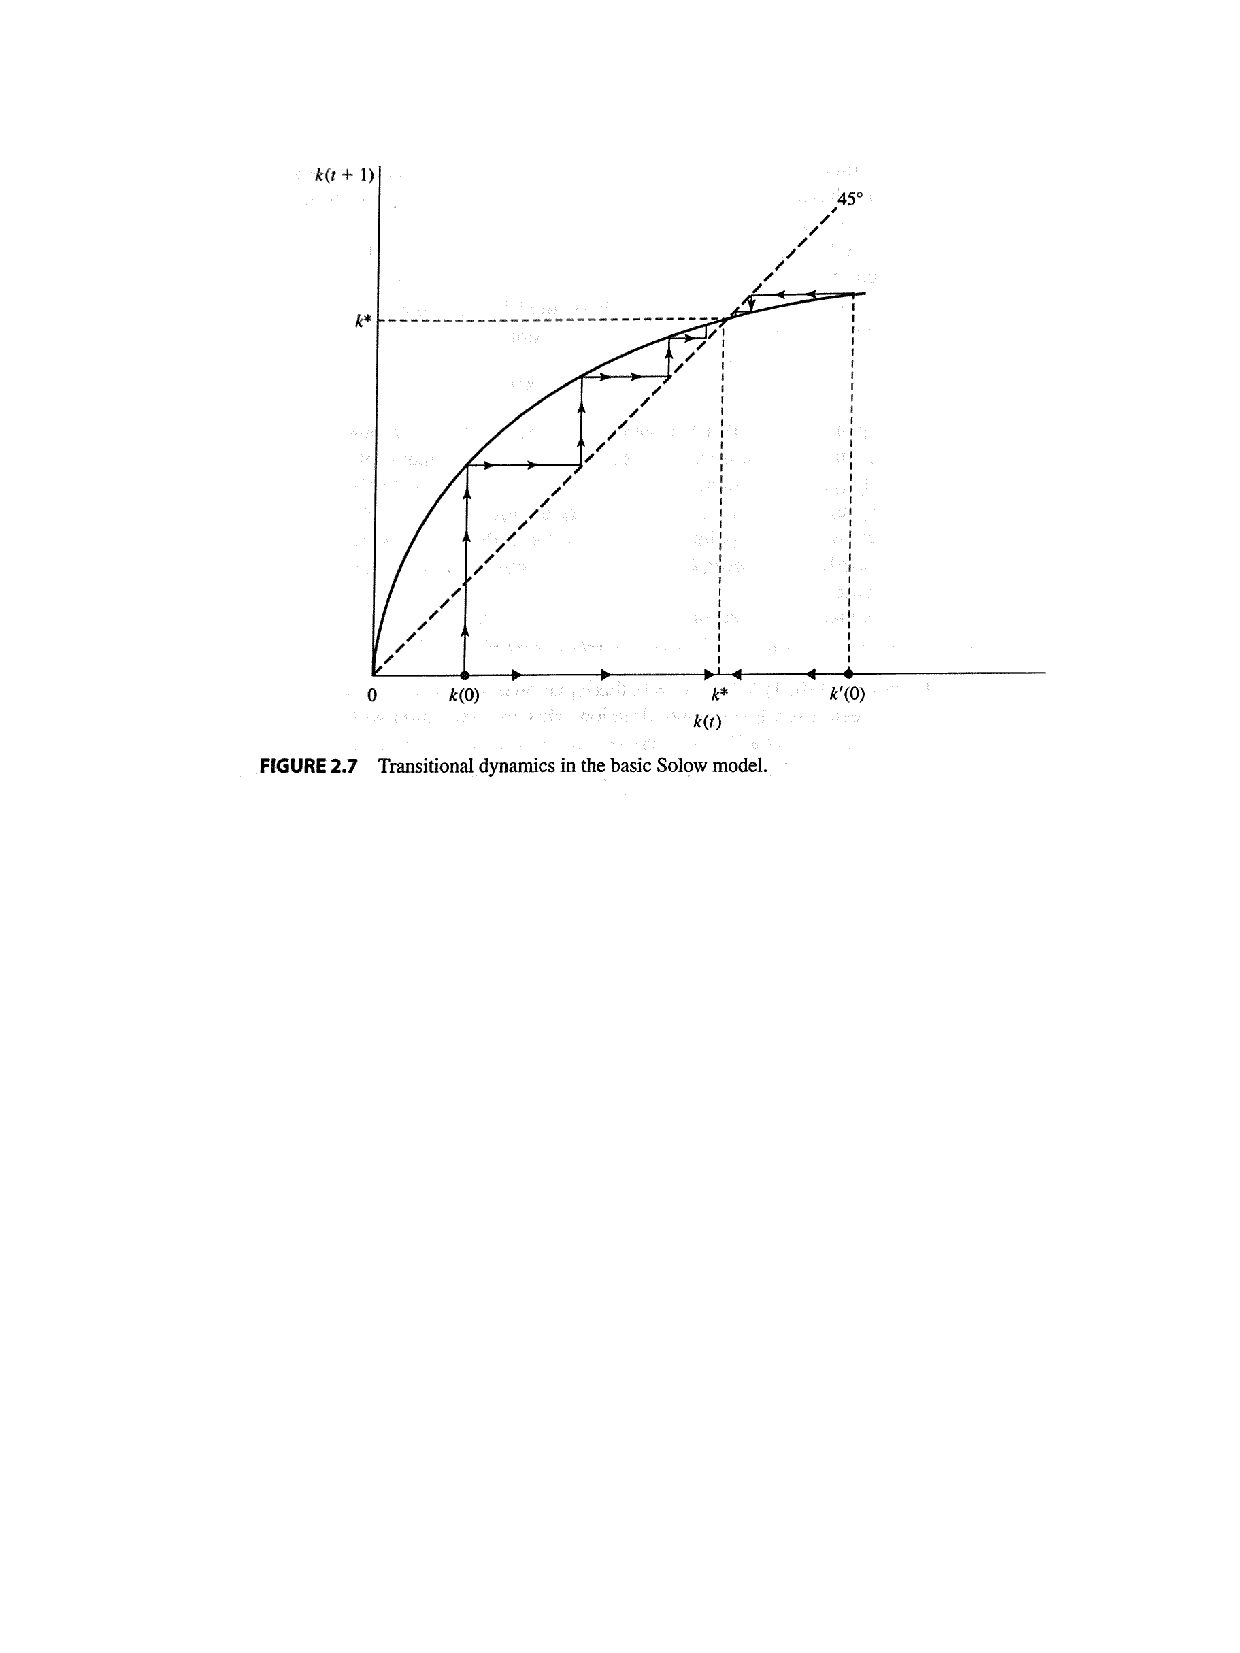
\includegraphics[scale=0.5]{./solow_transition_acemoglu.pdf}
\end{figure}
\end{frame}



%%%%%%%%%%%%%%%%%%%%%%%%%%  SLIDE   %%%%%%%%%%%%%%%%%%%%%%%%%%%%%%%%
\begin{frame}{6. Stochastic Difference Equations}
\begin{itemize}
\item Consider the process $\{X_t\}$ with 
\begin{equation}\label{eq:stochastic_difference}
	X_{t+1} = A X_t + Cw_{t+1}
\end{equation}
where $w_{t+1}$ is an iid. process with $w_{t+1} \sim \mathcal N(0, 1)$

\item Equation \eqref{eq:stochastic_difference} is a \textit{first-order, linear stochastic difference equation}

\item Let $\mathbb E_t$ the \textit{conditional expectation} operator (conditional on time $t$ information)

\item For example:
\begin{align*}
	\mathbb E_t(X_{t+1}) &= \mathbb E(X_{t+1} \mid X_t) = \mathbb E(A X_t + Cw_{t+1} \mid X_t) \\
	&= A X_t + C \mathbb E(w_{t+1} \mid X_t) = A X_t + C \mathbb E(w_{t+1}) = A X_t
\end{align*}
\end{itemize}
\end{frame}


%%%%%%%%%%%%%%%%%%%%%%%%%%  SLIDE   %%%%%%%%%%%%%%%%%%%%%%%%%%%%%%%%
\begin{frame}{}
\begin{itemize}
\item Rational expectations: agents' beliefs about stochastic processes are consistent with the true distribution of the process

\item Key equation: wealth dynamics with income fluctuations:
\begin{equation*}
	a_{t+1} = R_t a_t + y_t - c_t,
\end{equation*}
where $y_t$ is a stochastic process

\item Consumption Euler equation with uncertainty (e.g., stochastic income):
\begin{equation*}
	u'(C_t) = \beta R \mathbb E_t \Big[ u'(C_{t+1}) \Big]
\end{equation*}

\item New Keynesian Phillips curve with uncertainty (e.g., demand shocks):
\begin{equation*}
	\pi_t = \beta \mathbb E_t \Big[ \pi_{t+1} \Big] + \kappa x_t
\end{equation*}
\end{itemize}
\end{frame}










%%%%%%%%%%%%%%%%%%%%%%%%%%%%%%%%%%%%%%%%%%%%%%%%%%%%%%%%%%%%%%
%%%%%%%%%%%%%%%%%%%%%%%%%%%%%%%%%%%%%%%%%%%%%%%%%%%%%%%%%%%%%%
%%%%%%%%%%%%%%%%%%%%%%%%%%%%%%%%%%%%%%%%%%%%%%%%%%%%%%%%%%%%%%

\appendix


\end{document}









